Myonen lassen sich mit Hilfe eines Szintilationsdetektors nachweisen.
Die energiereichen Myonen geben einen Teil ihrer Energie an Szinitilationsmoleküle ab.
Diese kommen in einen angeregten Zustand.
Beim Rücksprung in den Grundzustand wird ein Photon emittiert.
Es besteht die Wahrscheinlichkeit, dass ein Myon im Szinitlatormaterial ebenfalls nach der Gleichung \ref{eqn:mu-}
oder \ref{eqn:mu+} zerfällt.
Das so entstandene Elektron besitzt genug kinetische Energie um seinerseits Atome anzuregen und so ebenfalls Photonen zu erzeugen.
Mit dem Abstand dieser beiden Lichtimpulse lässt sich die Lebensdauer einen Myons bestimmen.

\subsection{Aufbau}
Der Szintilationsdetektor besteht aus einem Edelstahlzylinder welcher ca. \SI{50}{l} fassen kann.
Um eine gute Zeitauflösung zu bekommen wird als Szintilatormaterial ein organisches Material benutzt,
da dieses schnell in seinen Grundzustand zurückspringt.
Die Abklingdauer des Szintilatormaterials beträgt ca. \SI{10}{s} und liegt damit unterhalb der Lebensdauer von Myonen.
Die einzelnen emittierten Photonen werden mit einem Sekundärelektronenvervielfacher(SEV) messbar gemacht.
Diese sind an beiden Seiten des Szintilators befestigt und werden mit Hochspannung betrieben.
Der elektrische Impuls, welcher durch das eindringen eines Myons ins Szintilatormaterial
und durch das Zerfallen dieses Myons im Szintilatormaterial entsteht,
wird an ein Zeit-Amplituden-Konverter (TAC) weitergegeben.
Dieser misst die Zeit zwischen den Signalen und gibt diese als Impulshöhe aus.
Mit Hilfe eines Multichannelanalyser werden die Impulshöhen der Häufigkeit nach sortiert.

Da einige Störfaktoren hinzukommen muss die Apparatur erweitert werden.
Im SEV können sich einzelnen Elektronen lösen und ebenfals ein Signal implizieren.
Die Amplitude dieser Rauschsignale ist hingegen meist geringer und kann so mit einer Diskriminatorschwelle herausgefiltert werden.
Der Diskriminator normiert die eingehenden Signale zusätzlich auf eine einheitliche Höhe und Länge.
Die Länge der Signale wird so gewählt dass ein Gangunterschied der Photonen im Szintilator ausgeglichen werden kann.
Eine weitere Möglichkeit der Rauschunterdrückung wird mit einer Koinzidenzschaltung verwirklicht.
Ein emittiertes Photon wird von beiden SEV gemessen.
Die resultierende Impulse werden über separate Kabel und Diskriminatoren in eine Koinzidenzschaltung geführt.
Da die Leitfähigkeit elektrischer Bauteile variieren kann,
können mit einer Verzögerungsleitung die Impulse aufeinander abgepasst werden.
Dafür werden die Verzögerungszeiten verändert und die resultierenden Impulse hinter der Koinzidenzschaltug gemessen.
Für die passende Verzögerungszeit ist die Impulsanzahl über eine bestimmte Messzeit maximal.
Der Koinzidenzschalter gibt nur dann ein Signal weiter wenn an beiden Eingängen ein Impuls ankommt.
Da die Myonen nich zwangsläufig in der mitte des Szintillators zerfallen kann es so ebenfalls zu einem minimalen Gangunterschied kommen.
Mit Hilfe der Diskriminatoren wird der eingehende Impuls verlängert sodass der Gangunterschied ausgeglichen werden kann.
Die Wahrscheinlichkeit, dass beide SEV gleichzeitig ein stakes Rauschsignal empfangen ist sehr gering.

Ein weiteres Problem ist, dass nur ein kleiner Teil der Myonen welche in der Szintilator eindringen dort auch zerfallen.
Das bedeutet das der TAC ein Startsignal bekommt, aber kein Stopsignal.
Da bei unendlich langer Suchzeit ein neu eintreffendes Myon ein Stopsignal geben würde, anstatt ein neues Startsignal,
muss die Suchzeit $\text{T}_{\text{S}}$ nach einer gewissen Zeit abgebrochen werden.
Der Suchzeitgeber wird mit einer monostabilen Kippstufe oder auch Univibrator verwirklicht.
Nach Aktivierung bleibt die Kippstufe über die Zeit $\text{T}_{\text{S}}$ in einem angeregen Zustand und spring dann in seinen Grundzustand zurück.
Die monostabiele Kippstufe besitzt zwei Ausgänge (OUT) wobei einer dieser Ausgänge $\overline{\text{OUT}}$ invers ist.
Im Grundzustand wird also über den OUT-Ausgang kein Signal weiter gegeben (Logisch 0).
Der Ausgang $\overline{\text{OUT}}$ gibt hingegen ein Signal weiter (Logisch 1).
Die beiden Ausgänge werden wie auf dem Schaltbild \ref{fig:block} mit den AND-Gattern 1 und 2 verbunden.
Die AND-Gatter geben nur dann ein Signal weiter wenn an beiden ihrer Eingänge ein Signal (Logisch 1) anliegt.

\begin{figure}[h!]
  \centering
  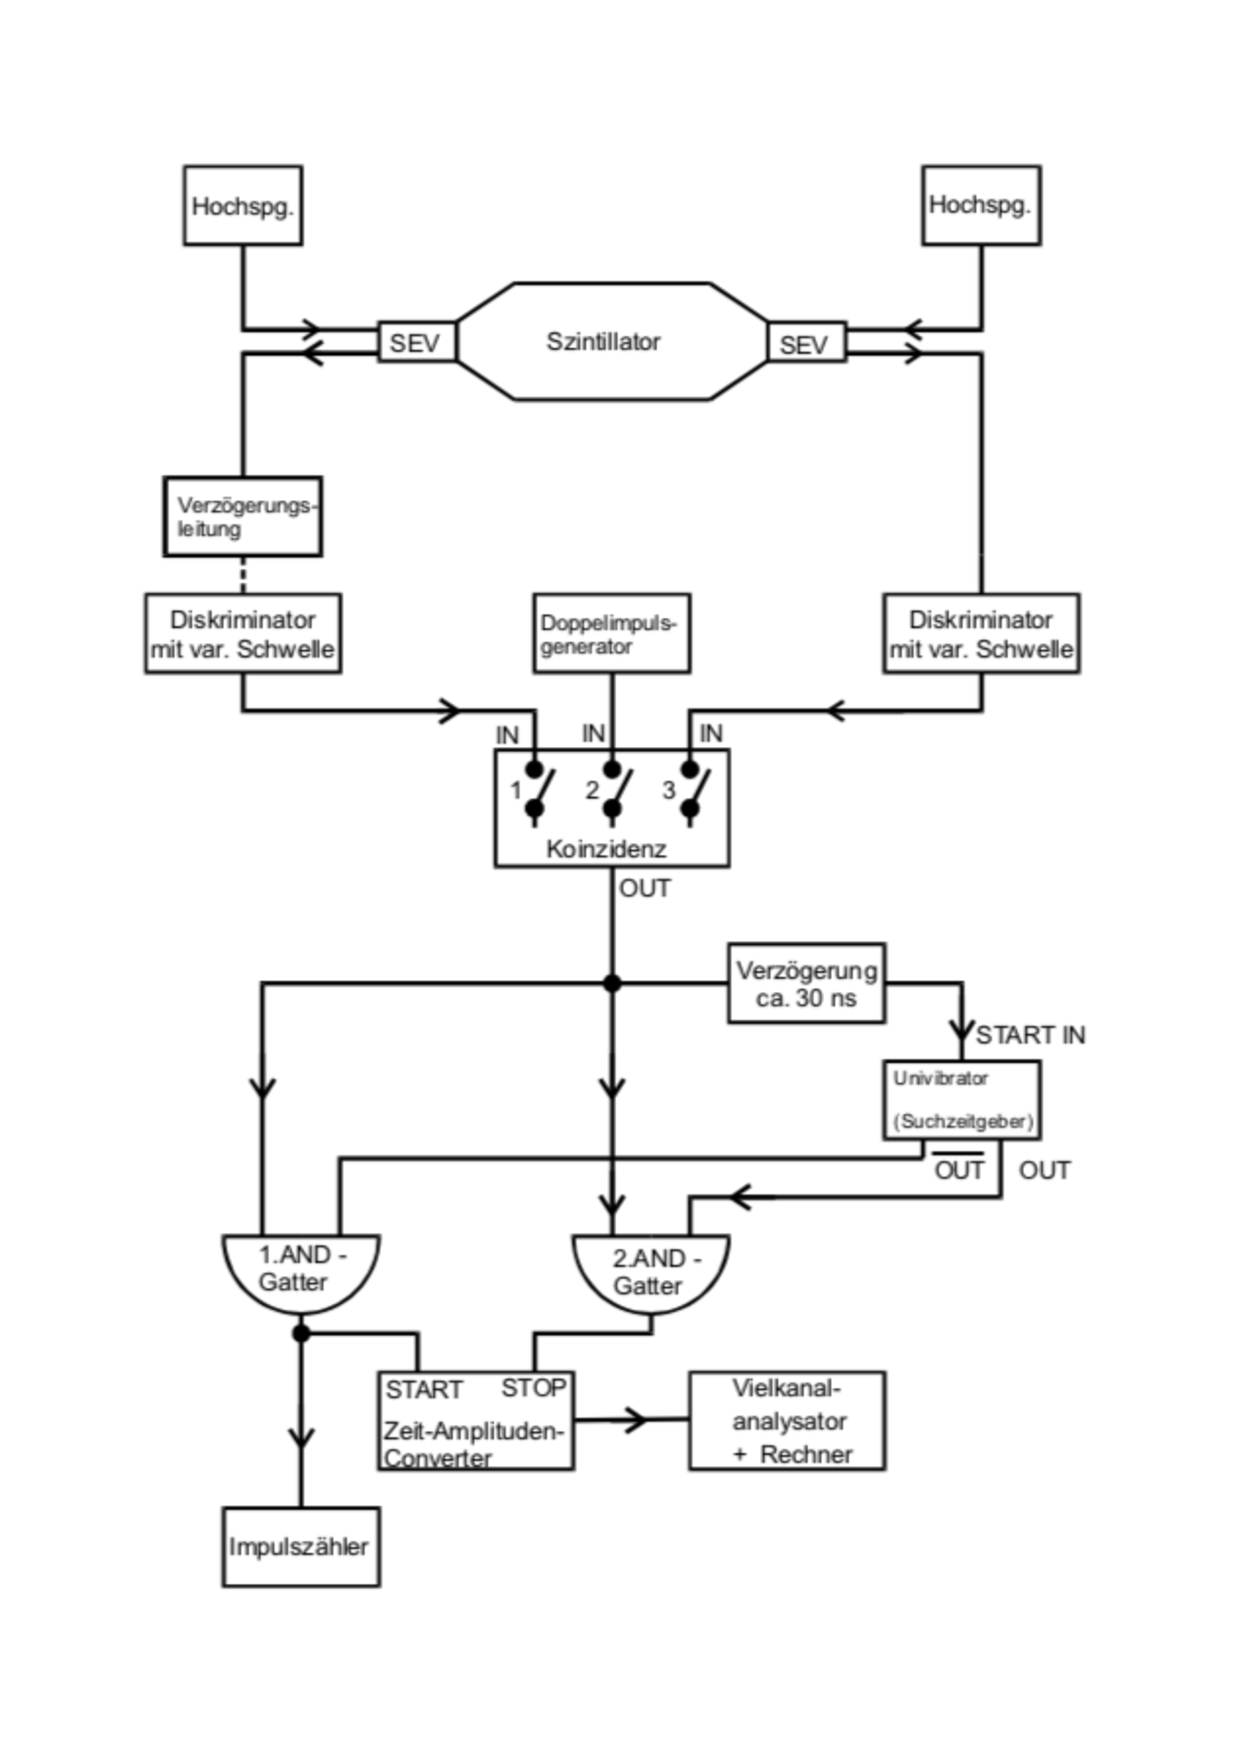
\includegraphics[width=0.6 \textwidth]{schaltung.pdf}
  \caption{Blockschaldbild der Messapperatur}
  \label{fig:block}
\end{figure}
\FloatBarrier

Nach der Koinzidenzschaltung wird das Signal also in drei Teile aufgeteilt.

Zum einen wird ein Signal zum 1 AND-Gatter weiter geleitet.
Dort liegt nun das Signal vom Myon und das Signal von der monostabielen Kippstufe ($\overline{\text{OUT}}$) an.
Das Signal wird also vom 1 AND-Gatter durchgelassen und gibt somit das Startsignal für den TAC.
Das Signal wird ebenfalls mit einem Impulszähler aufgenommen.

Zum anderen wird das Signal an den 2 AND-Gatter weiter gegeben.
Das eingehende Signal wird jedoch nicht weiter gegeben, da am zweiten Eingang kein Signal von der monostabielen Kippstufe kommt.

Als letztes wird das Signal über einen Verzögerer zur monostabielen Kippstufe geleitet.
Diese wird angeregt und Verändert so über den Suchzeitraum $\text{T}_{\text{S}}$ das Ausgangssignal.
Es wird also an $\overline{\text{OUT}}$ kein Signal (Logisch 0) und an OUT Logisch 1 abgegeben.

Kommt nun das Signal über den Zerfall des Myon kann das Signal den 1 AND-Gatter nicht passieren, das 2 AND-Gatte hingegen schon.
Somit wird das Signal als Stopsignal für den TAC gewertet.
Zusätzlich wird auch dieses Signal mit einem Impulszähler erfasst.
Das vom TAC konvertierte Signal wird über einen Vielkanalanalysator in einem Computerprogramm verarbeitet.

Zerfällt das Myon nicht im Szintilator bleibt das Signal über den Zerfall aus.
Daraufhin springt die monostabiele Kippstufe nach der Zeit $\text{T}_{\text{S}}$ in den Grundzustand zurück.
Ein neu ankommendes Myon löst somit wieder ein Startsignal aus.
$\text{T}_{\text{S}}$ sollte demendsprechend so gewählt werden, dass die Suchzeit größer ist als die Lebensdauer eines Myons
aber kleiner als die warscheinliche Wiedereintrittszeit eines neuen Myons.

\subsection{Durchführung}
Es wird die Schaltung wie in der Abbildung \ref{fig:block}.
Zusätzlich wird die Anzahl der Stopimpule mit einem Impilszähler ermittelt.

Um die passende Verzögerungszeit $\text{T}_{\text{VZ}}$ zu ermitteln muss, wie bereits beschieben, die Zeit Variiert werden.
Misst man hinter der Koinzidenzschaltung die Impulse kann so eine abhängigkeit von $\text{T}_{\text{VZ}}$ und der anzahl der Impules festgestellt werden.
$\text{T}_{\text{VZ}}$ ist richtig gewählt wenn die Impulsanzahl maximal ist.

Die Diskriminatoren werden so eingestellt, dass der Großteil des Rauschens unterdrückt wird die Impules welche von den Myonen stammen jedoch passieren konnen.
Die Impulslänge wird auf ca. $\SI{4}{ns}$ gestellt um den möglichen Gangunteschied des Lichtes im Szintillator auszugleichen.

Die Suchzeit $\text{T}_{\text{S}}$ der monostabielen Kippstufe wird so eingestellt das die Suchzeit größer ist als Lebensdauer der Myonen jedoch kleiner ist als
der warscheinlich nächste Eintritt eines Myons in die Messaperatur.
Mithilfe eines Doppelimpulsgeneratort kann die Funktionsweise der monostabielen Kippstufe überprüft werden.
Da es trotzdem sein kann, dass ein neu angekommenes Myon die Messung eines Vorherigen beendet und so ein falsches Stopsignal erzeugt, muss von den Messwerten eine bestimmte Untergrundstrahlung abgezogen werden.

Da die Anzahl der in Messaperatur zerfallenen Myonen klein ist gegen die Anzahl der Myonen muss die gesamte Messung über einen Zeitraum von ca. $\SI{20}{h}$ erfolgen.
